\documentclass[border={0pt 0pt}]{standalone}

\renewcommand{\familydefault}{\sfdefault}

\usepackage[rgb]{xcolor}

\colorlet{fgcolor}{black}
\colorlet{bgcolor}{white}

\newcommand{\saturation}{0.45}
\newcommand{\brightness}{0.75}

\definecolor{myblue}{Hsb}{200,\saturation,\brightness}
\definecolor{myorange}{Hsb}{30,\saturation,\brightness}
\definecolor{myred}{Hsb}{350,\saturation,\brightness}
\definecolor{mygreen}{Hsb}{115,\saturation,\brightness}
\colorlet{mygray}{gray!50!bgcolor}

\usepackage{tikz}
\usepackage{tikz-timing}
\usetikzlibrary{fit, positioning, shapes.geometric, shapes.symbols, backgrounds}

\newlength{\vhdlregh}\setlength{\vhdlregh}{2em}
\newlength{\vhdlregw}\setlength{\vhdlregw}{1em}

\tikzset{
    text=fgcolor,
    arrow/.style={ ->, draw=fgcolor, very thick },
    % Register
    regbox/.style={ rectangle, very thick, draw=fgcolor, fill=mygray, minimum width=\vhdlregw, minimum height=\vhdlregh },
    regwedge/.style={ isosceles triangle, isosceles triangle apex angle=80, draw=fgcolor, very thick, anchor=right corner, scale=0.33 },
    register/.pic={
        \node[regbox] () {#1};
        \node[above right=0.1em and 0.05em of .south west, regwedge] (-wedge) {};
    },
    % Wire bitwidth marker
    pics/bitwidth/.style args={#1/#2}{code = {
        \coordinate (-middle);
        \coordinate[above left=4pt of -middle] (-start);
        \coordinate[below right=4pt of -middle] (-end);
        \draw[fgcolor, thick] (-start) to (-end);
        \node[#2=1pt of -middle] {{\footnotesize #1}};
    }},
    % Adder, multiplier, etc.
    adder/.style={ circle, draw=fgcolor, very thick },
    % Cloud (for combinational logic)
    mycloud/.style={ cloud, draw=fgcolor, very thick, inner sep=2pt, minimum width=0.8cm, minimum height=0.8cm },
    subcomponent/.style={ draw=fgcolor, densely dotted, very thick, rounded corners, inner sep=1em }
}


\usepackage{bm}

\begin{document}

\pagecolor{bgcolor}

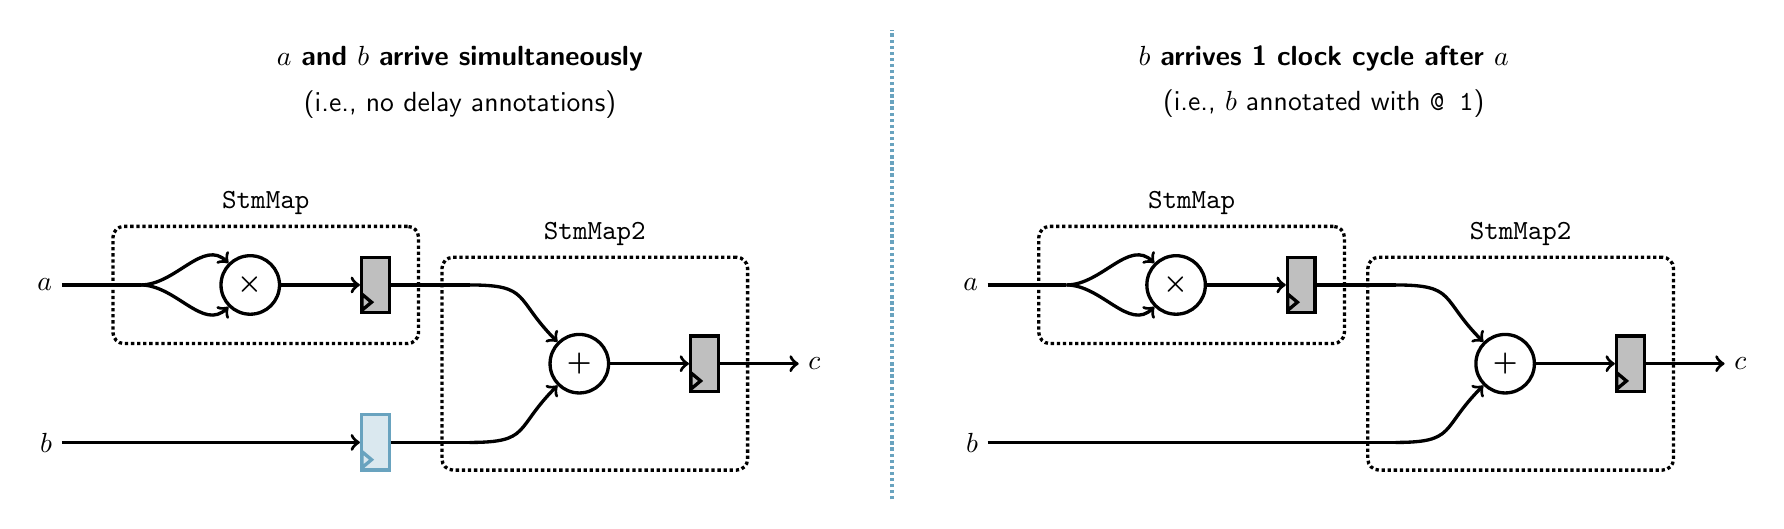
\begin{tikzpicture}
    % ===== Before adding delay annotation =====================================
    \coordinate (before-start);
    \coordinate[above=of before-start] (before-start-above);
    \coordinate[below=of before-start] (before-start-below);
    \node[left=0pt of before-start-above] {$a$};
    \node[left=0pt of before-start-below] {$b$};

    % StmMap
    \coordinate[right=of before-start-above] (before-square-input);
    \node[adder, right=of before-square-input] (before-square) {$\boldsymbol{\times}$};
    \pic[right=of before-square] (before-square-reg) {register};
    \node[subcomponent, fit=(before-square-input) (before-square) (before-square-reg)] (before-square-subcomponent) {};
    \node[above=0pt of before-square-subcomponent] {\texttt{StmMap}};

    % Register added for latency matching
    \coordinate (before-latmatch-reg) at (before-square-reg.west|-before-start-below);
    \begin{scope}[
        regbox/.append style={ draw=myblue, fill=myblue!25!bgcolor },
        regwedge/.append style={ draw=myblue, fill=myblue!25!bgcolor },
    ]
        \pic[below=0pt of before-latmatch-reg, anchor=west, draw=myblue, fill=myblue!50!bgcolor] (before-latmatch-reg) {register};
    \end{scope}

    % StmMap2
    \coordinate[right=of before-square-reg] (before-above);
    \coordinate (before-below) at (before-above|-before-start-below);
    \draw[transparent] (before-above.east) to coordinate[midway] (midway) (before-below.east);
    \node[adder, right=of midway] (before-zip) {$\boldsymbol{+}$};
    \pic[right=of before-zip] (before-zip-reg) {register};
    \node[right=of before-zip-reg] (before-end) {$c$};
    \node[subcomponent, fit=(before-below) (before-above) (before-zip) (before-zip-reg)] (before-zip-subcomponent) {};
    \node[above=0pt of before-zip-subcomponent] {\texttt{StmMap2}};

    % Arrows
    \draw[arrow, -] (before-start-above) to (before-square-input);
    \draw[arrow, out=0, in=135] (before-square-input) to (before-square.north west);
    \draw[arrow, out=0, in=225] (before-square-input) to (before-square.south west);
    \draw[arrow] (before-square) to (before-square-reg);
    \draw[arrow, -] (before-square-reg) to (before-above);
    \draw[arrow] (before-start-below) to (before-latmatch-reg);
    \draw[arrow, -] (before-latmatch-reg) to (before-below);
    \draw[arrow, out=0, in=135, looseness=1.5] (before-above) to (before-zip);
    \draw[arrow, out=0, in=225, looseness=1.5] (before-below.east) to (before-zip);
    \draw[arrow] (before-zip) to (before-zip-reg);
    \draw[arrow] (before-zip-reg) to (before-end);

    % ===== After adding delay annotation ======================================
    \coordinate[right=2 of before-end] (after-start);
    \coordinate[above=of after-start] (after-start-above);
    \coordinate[below=of after-start] (after-start-below);
    \node[left=0pt of after-start-above] {$a$};
    \node[left=0pt of after-start-below] {$b$};

    % StmMap
    \coordinate[right=of after-start-above] (after-square-input);
    \node[adder, right=of after-square-input] (after-square) {$\boldsymbol{\times}$};
    \pic[right=of after-square] (after-square-reg) {register};
    \node[subcomponent, fit=(after-square-input) (after-square) (after-square-reg)] (after-square-subcomponent) {};
    \node[above=0pt of after-square-subcomponent] {\texttt{StmMap}};

    % StmMap2
    \coordinate[right=of after-square-reg] (after-above);
    \coordinate (after-below) at (after-above|-after-start-below);
    \draw[transparent] (after-above.east) to coordinate[midway] (midway) (after-below.east);
    \node[adder, right=of midway] (after-zip) {$\boldsymbol{+}$};
    \pic[right=of after-zip] (after-zip-reg) {register};
    \node[right=of after-zip-reg] (after-end) {$c$};
    \node[subcomponent, fit=(after-below) (after-above) (after-zip) (after-zip-reg)] (after-zip-subcomponent) {};
    \node[above=0pt of after-zip-subcomponent] {\texttt{StmMap2}};

    \draw[arrow, -] (after-start-above) to (after-square-input);
    \draw[arrow, out=0, in=135] (after-square-input) to (after-square.north west);
    \draw[arrow, out=0, in=225] (after-square-input) to (after-square.south west);
    \draw[arrow] (after-square) to (after-square-reg);
    \draw[arrow, -] (after-square-reg) to (after-above);
    \draw[arrow, -] (after-start-below) to (after-below);
    \draw[arrow, out=0, in=135, looseness=1.5] (after-above) to (after-zip);
    \draw[arrow, out=0, in=225, looseness=1.5] (after-below.east) to (after-zip);
    \draw[arrow] (after-zip) to (after-zip-reg);
    \draw[arrow] (after-zip-reg) to (after-end);

    % ===== Separator ==========================================================
    \draw[transparent] (before-end) to coordinate[midway] (vrule-mid) (after-start);
    \coordinate[above=5em of current bounding box.north] (vrule-top);
    \coordinate[below=5pt of current bounding box.south] (vrule-bot);
    \draw[arrow, -, myblue, densely dotted] ([xshift=0pt, yshift=-5pt] vrule-bot) to ([xshift=0pt, yshift=5pt] vrule-top);

    % "Before" title
    \draw[transparent] (current bounding box.north west) to coordinate[midway] (before-title) (vrule-top);
    \node[below=0pt of before-title] (before-title) {\textbf{$a$ and $b$ arrive simultaneously}};
    \node[below=0pt of before-title] (before-title) {(i.e., no delay annotations)};

    % "After" title
    \draw[transparent] (current bounding box.north east) to coordinate[midway] (after-title) (vrule-top);
    \node[below=0pt of after-title] (after-title) {\textbf{$b$ arrives 1 clock cycle after $a$}};
    \node[below=0pt of after-title] (after-title) {(i.e., $b$ annotated with \texttt{@ 1})};
\end{tikzpicture}

\end{document}
